\chapter{数据集的构建和预处理}

上一章节提到了验证工具的检测能力需要大量的测试用例,由于合适开源用例的稀缺,合理利用现有无缺陷代码来生成空指针引用缺陷是一种可行的方法。但是,为了方便后续的处理工作,测试用例的选择应该从多维度慎重考虑。然后,为了模型训练的顺利进行,还需要对这些数据进行预处理,构建出正确的控制流图,提取出合适的代码特征。这些工作都是神经网络模型训练所依赖的重要基础。

\section{数据集构建}
\subsection{数据来源}
如果采用从正常代码中构建空指针引用缺陷的方式,首先面对的问题就是选择构建用例的合适的原材料。为了便于后期处理,用例应该包含程序入口,具备语义完整,结构多样化,代码规范简洁等特点,只要程序包含常见的语法结构和调用关系,程序规模不应过大,恰好包含空指针引用陷产生的上下文最佳。依据这些条件,本文选择了部分开源代码数据集作为构建空指针引用缺陷的原始资料,如图\ref{fig:figure4-1}所示。

\begin{figure}
	\centering
	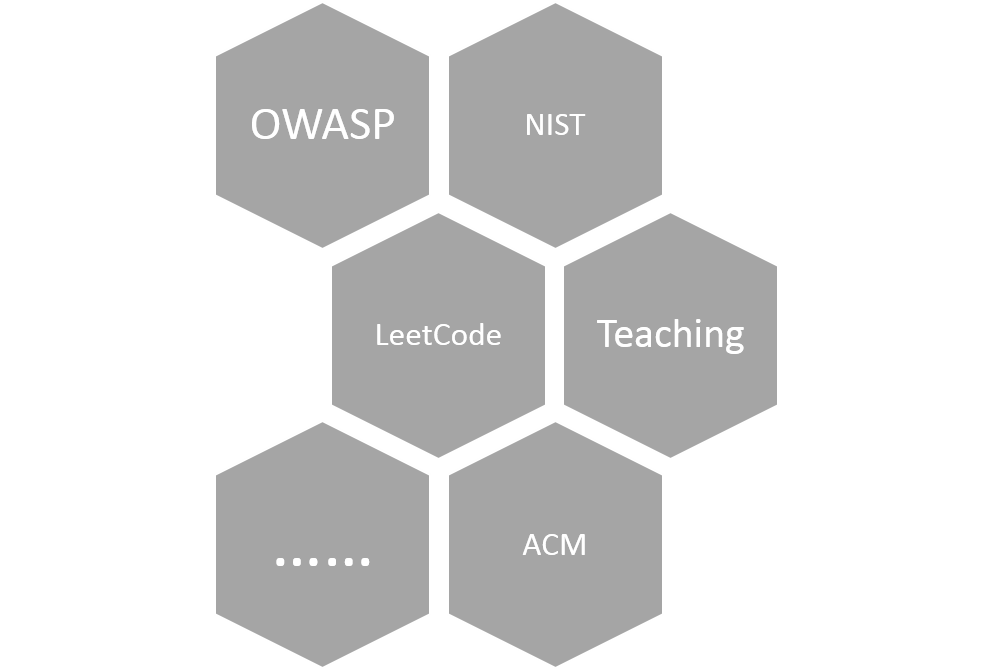
\includegraphics[width=0.70\textwidth]{figures/resource4-1}
	\caption{测试用例来源}\label{fig:figure4-1}
\end{figure}

其中,OWASP[+]和ONIST[+]分别为代码缺陷检测相关领域的项目,从这些项目下可以获得部分标准的空指针引用缺陷用例,同时也可以得到很多具备其他缺陷的测试用例,由于这些用例的代码编写较为规范,并且经过了合理分类,还往往包含说明文档等辅助理解代码的信息,大多都可以用来生成空指针引用缺陷。除此之外,LeetCode和ACM作为编程竞赛性质的项目下也包含大量可以利用的代码,这些代码根据题目的难易级别具备着不同的复杂程度,包含了多样的代码结构,同时,代码的规模往往不大,是作为测试用例生成的良好材料。另外,一些供教学使用的代码也是十分合适的空指针缺陷构造来源,作为补充,本文还添加了部分人工编写的测试用例。

\subsection{测试用例生成}
在取得构造测试用例的原始代码后,需要对这些代码进行检查,确保代码有正确的程序入口,并且可以正确执行。对于OWASP和ONIST项目下的代码,很多用例缺乏Main方法的入口,这会导致后续控制流图提取的困难,这时需要在源代码层级加入合适main方法,调用合适的方法驱动程序的执行。此外,对于ACM和LeetCode项目下的代码资源,虽然所有用例都包含正确的程序入口,但是往往需要合适的输入数据程序才能正确执行。获得这些用例的输入数据并不困难,只需要按照相应题目下的输入输出样子给予输入数据即可驱动程序执行,这些数据的获取可以通过爬虫程序取得,输入数据则可以通过重定向程序的输入流来完成。

空指针引用缺陷的产生必然需要一个产生Null值的缺陷源,在程序的某个位置,变量被赋值为Null随后沿着控制流图向前传播,在遇到解引用时便会触发空指针引用异常。这个变量便是缺陷源,只要在程序中的合适位置构造缺陷源,则有一定的可能会在程序的下文中触发空指针引用缺陷。当用例的可用性得到确认后,需要对用例程序进行语法分析,寻找合适的空指针产生点并构造缺陷源。

对Java文件进行语法分析可以使用Eclipse JDT下的AST来完成,该工具可以在Eclipse环境下获得,利用它能够对Java文件进行解析,生成相应的抽象语法树,并且能够任意修改Java代码的结构和内容。在AST中,Java代码的每一个语法结构都有对应的AST结点表示,这些结点具有完整的层次结构,可以表示整个程序对象到具体方法的某个具体变量。如图\ref{fig:figure4-2}所示,一个for循环的代码片段按照Eclipse AST的标准解析出抽象语法树,表\ref{tab:table4-1}表示部分结点在AST树中对应的名称。

\begin{figure}
	\centering
	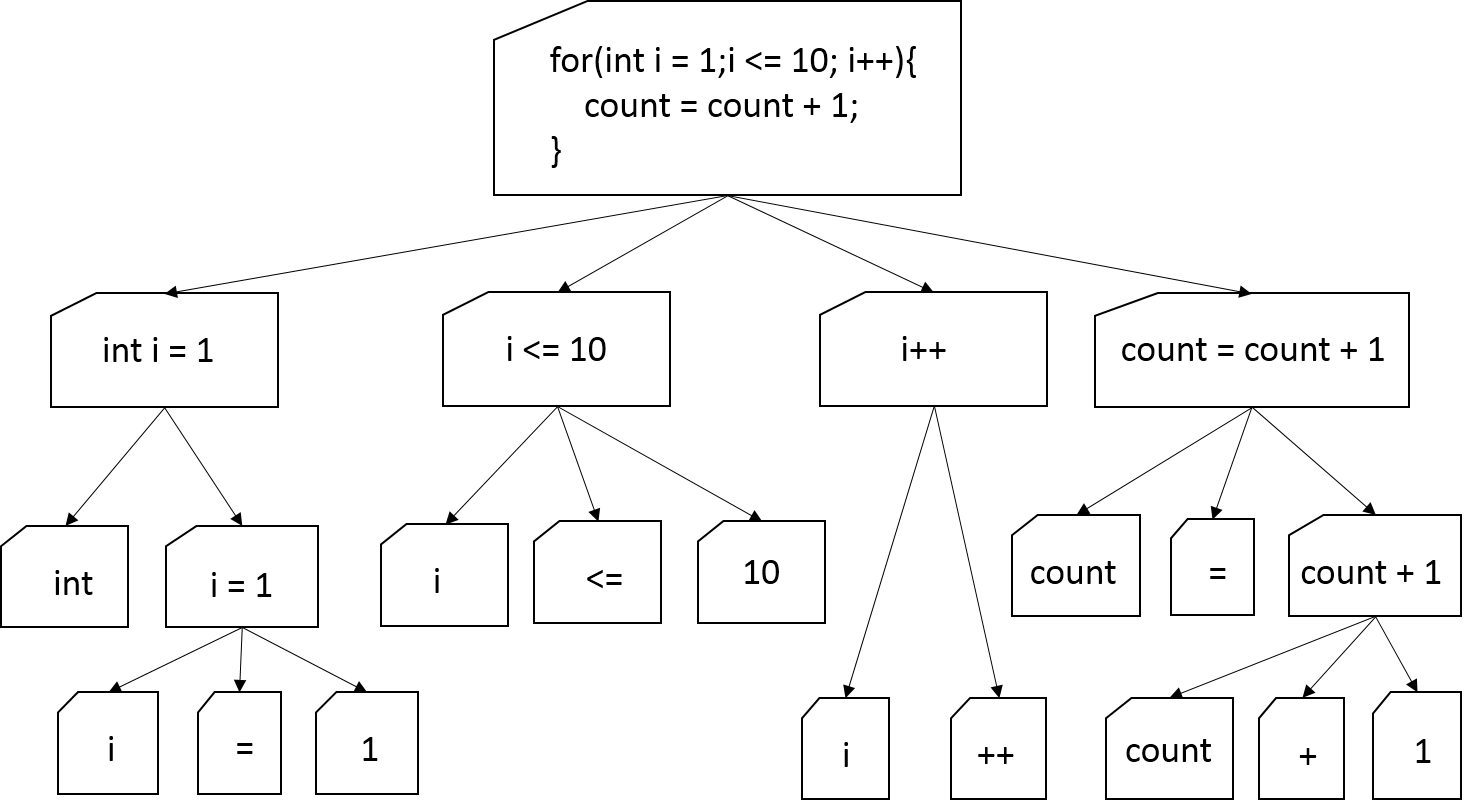
\includegraphics[width=0.70\textwidth]{figures/ast4-2}
	\caption{抽象语法树示例}\label{fig:figure4-2}
\end{figure}

\begin{table}
	\centering
	\caption{AST中的结点信息} \label{tab:table4-1}
	\begin{tabular*}{0.9\textwidth}{@{\extracolsep{\fill}}ccc}
		\toprule
		子节点	&子节点名	&依附于父结点的角色 \\
		\midrule
		int i = 1	&VariableDeclarationExpression	&INITIALIZERS \\
		i <= 10	&InfixExpression	&EXPRESSION \\
		i++	&PostExpression	&UPDATERS \\
		{ count = count + 1 }	&Block	&BODY \\
		\bottomrule
	\end{tabular*}
\end{table}

在生成用例的抽象语法树后,只要找到合适的点位,就可以通过修改合适的操作数为Null来构造空指针引用缺陷源。通常这些点位都和赋值表达式有关,但是在过程间调用的上下文中,方法的参数和返回值都可以是合适的构造点位。可以利用的修改位置有:

(1)类的属性成员。

(2)方法内的局部变量。

(3)方法的参数。

(4)方法的返回值。

其中(1)中的属性成员包含被初始化的非Null的普通属性和静态属性。(1)和(2)需要找到相关的赋值表达式,通过修改右操作数为Null来生成空指针引用缺陷源。(3)需要判断被调用方法的参数列表中属性的类型,将引用类型的实参修改为Null即可。(4)需要判断该方法的返回值类型,只有返回值为引用类型才可以修改。

图\ref{fig:figure4-3}为测试用例构建的流程图,在抽象语法树的基础上进行修改获得缺陷源后,需要对程序进行编译并执行才能确定能否真正构建出空指针引用缺陷用例,如果没有通过编译或者运行后没有发生空指针引用缺陷,则用例构造失败,需要重新寻找新的构建点位。重复此步骤直到成功产生空指针引用缺陷。最后,成功构建的缺陷用例需要在代码中添加代码信息的注解表明该缺陷的缺陷源和发生空指针解引用的位置。运用注解的方式是为了后续代码信息抽取的工作顺利进行,Java程序可以很方便地抽取代码的注解信息,而这些自定义注解不会对代码的实际语义产生影响。记录空指针解引用的位置是为了验证工具检测的结果,加上缺陷源的位置可以很方便的确定该空指针引用缺陷发生的上下文范围,确定分析域。这些注解信息需要放置在测试用例的Main方法所在类中,方便代码信息抽取时统一处理,如果缺陷的产生位置不在Main方法所在类的方法中,就需要在注解信息中表明该缺陷产生位置所在的类。

\begin{figure}
	\centering
	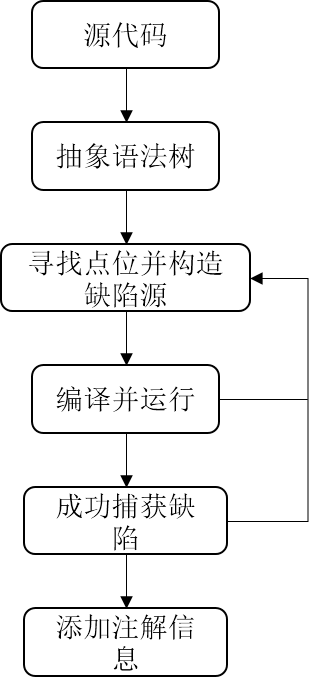
\includegraphics[width=0.25\textwidth]{figures/parse4-3}
	\caption{测试用例构建流程}\label{fig:figure4-3}
\end{figure}

下面的代码片段就展示了一个成功生成的测试用例,在代码的第8行将“sb = new StringBuilder("")”修改为“sb = null”,随后在代码的第11行即对sb进行解引用操作,触发空指针引用缺陷。在第一行的注解标注了该缺陷涉及的上下文代码行号及变量名,这表示了分析域的范围。这个例子非常简单,实际上产生的代码在复杂度上是满足要求的,选用的原始代码往往都具备跨方法和跨文件的调用关系。 

\begin{lstlisting}[language={[AspectJ]Java},numbers=left,keywordstyle=\color{blue!70},commentstyle=\color{red!50!green!50!blue!50},frame=shadowbox, rulesepcolor=\color{red!20!green!20!blue!20}] 
$@Context(start = 8, end = 11, var = “sb")$
public static void main(String[] args) {
      Scanner in = new Scanner(System.in); 
      int k = in.nextInt();
      if(k > 36){
           System.out.println("-1");
      }else{
          StringBuilder sb = null; //source                 
          int mul = k/2;
          while(mul-- > 0){
              sb.append("8"); //npe
          }
          if(k%2 == 1){
              sb.append("4");
          }
          System.out.println(sb.toString());
      }
}
\end{lstlisting}

\section{控制流图提取}
控制流图(Control Flow Graph,CFG)是一个程序或者过程的抽象表现,代表了程序执行过程中所有可能经历的路径信息,能准确刻画一份代码的结构信息。空指针引用缺陷测试用例生成完毕后,需要生成代码的控制流图。
\subsection{Soot}
Soot【生存手册第13个引用】是一种Java字节码优化框架,凭借着对Java语言强大的分析能力,已经被广泛地应用于很多针对Java语言的分析优化项目。Soot框架最大的特点就是它提供了四种不同的代码中间表示形式:Jimple,Baf,Grimp和Shimple,它们考虑到不同的分析场景,对代码进行了不同程度的抽象表示。同时,Soot还构建了数据结构来表示待分析的项目,如表\ref{tab:table4-2}所示。这些特有的表示方法使得代码的分析过程变得更加简单和灵活。Soot的工作过程如图\ref{fig:figure4-4}所示。

\begin{table}[hb]
	\centering
	\caption{Soot中表示项目的数据结构} \label{tab:table4-2}
	\begin{tabular*}{0.9\textwidth}{@{\extracolsep{\fill}}cc}
		\toprule
		类名	&描述	 \\
		\midrule
		Scene	&表示整个分析环境\\
		SootClass	&表示一个class	\\
		SootMethod	&表示一个Method	 \\
		SootField	&表示一个类成员属性	\\
		Body	&表示一个方法体 \\
		\bottomrule
	\end{tabular*}
\end{table}

\begin{figure}
	\centering
	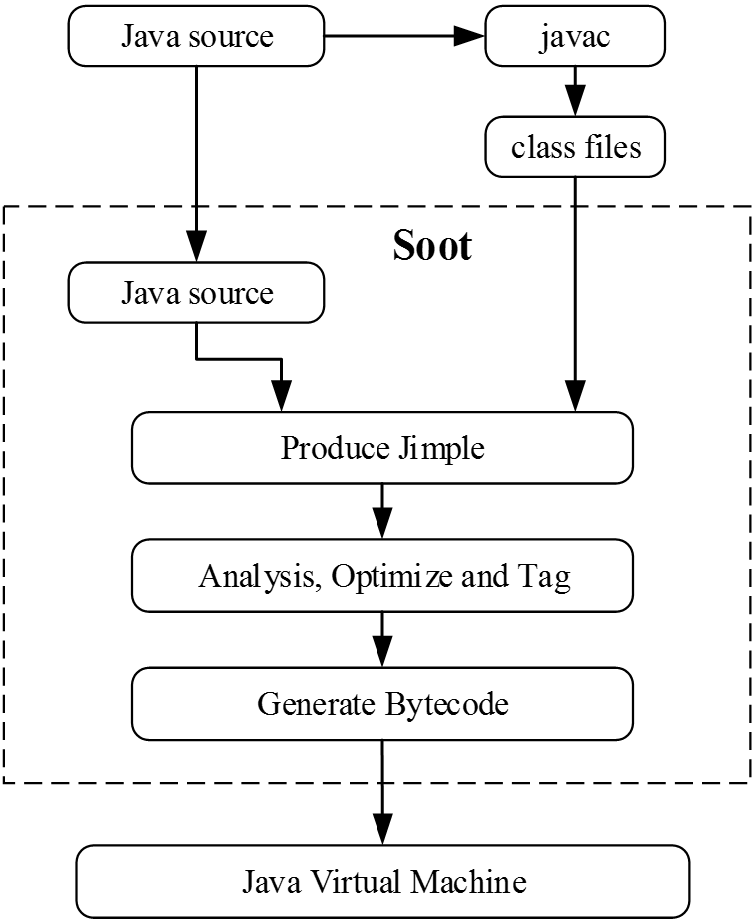
\includegraphics[width=0.70\textwidth]{figures/Soot4-4}
	\caption{Soot工作流程}\label{fig:figure4-4}
\end{figure}

Jimple是Soot框架中最主要的代码中间表示形式,采用了典型的基于三地址的语句表达形式,它可以由Java源代码或者Java字节码转换得到。其中,通过字节码的转换通过为隐式的堆栈变量引入新的局部变量以及清除jsr指令来完成。在代码转换的过程中,Jimple中的局部变量会被加上被推断出来的类型信息,同时部分没有用到的局部变量也会在优化阶段被清除掉从而不会出现在Jimple代码中,最重要的是代码中所有的表达式都会经过线性化的处理,最终Jimple将由若干三地址表达式组成,这些表达式至多包含三个变量或者常量信息,这种规则对于执行代码优化是非常方便的。另一方面,Jimple表示形式所包含的语句类型只有15条,相比于Java字节码中多达200多条的指令类型,Jimple的表示形式是足够简洁的,这些精简之后的指令类型也给本文后续的代码特征提取提供了极大的便利。

除了简洁准确的表示形式,利用Soot还可以进行复杂的别名分析和数据流分析。另外,每个待分析方法的方法体,即表\ref{tab:table4-2}中的Body,都包含了一个Units链,Unit是Soot中的一个接口,具体实现则是一个三地址表达式,这些表达式实际上会对应到Jimple中的某个具体语句类型,即Stmt。这些Unit已经包含了互相之间的结构关系,根据这些结构关系可以很方便地生成方法内的控制流图。同时,对于包含调用方法语句类型的Unit,通过Soot提供的API还可以很方便的得知该调用的对象方法,这对后面过程间调用图的构建非常重要。

\subsection{全局控制流图构建}
上一节介绍了Soot,利用它可以构建出方法内的控制流图和过程间的调用图,进而得到全局控制流图。

方法内的控制流图可以从以Jimple表示的方法体中包含的Units链得到。通过遍历Units链中的Unit元素,可以得到它们的前驱和后继结点,这些信息实际上就表示了该方法的控制流图,不过它的结点是一个Jimple表示的Stmt,在Jimple中表示了一种语句类型。如下面的代码片段所示,不同的语句对应着Jimple中不同的Stmt类型,这些类型有15种之多,是Jimple能够表示的最基本的语法单位。
\begin{lstlisting}[language={[AspectJ]Java},numbers=left,keywordstyle=\color{blue!70},commentstyle=\color{red!50!green!50!blue!50},frame=shadowbox, rulesepcolor=\color{red!20!green!20!blue!20}] 
public int foo(java.lang.String){//locals
    r0 := @this; // IdentityStmt
    r1 := @parameter0;
    if r1 != null goto label0; // IfStmt
    $\$$i0 = r1.length(); // AssignStmt
    r1.toUpperCase(); // InvokeStmt
    return $\$$i0; // ReturnStmt
label0: // createdbyPrinter
    return2;
}
\end{lstlisting}
从该代码块中可以抽取出foo方法包含的Units链,进而得到其结构信息,如图\ref{fig:figure4-5}所示,结点的序号为代码块中语句对应的行号。从图中任意一个结点都可以找到其相邻的前驱和后继结点,这种关系不是静态代码顺序的关系,其考虑了代码执行逻辑的语序。

\begin{figure}
	\centering
	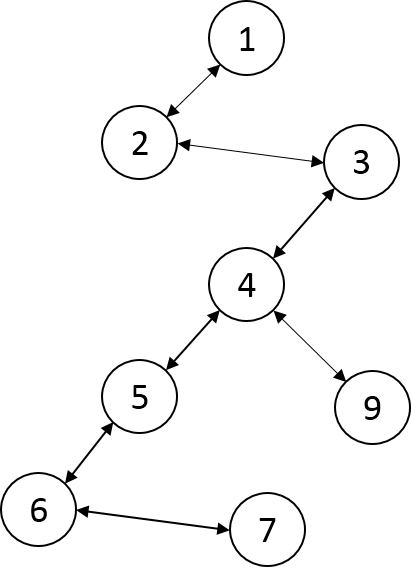
\includegraphics[width=0.25\textwidth]{figures/Units4-5}
	\caption{示例代码的Units关系图}\label{fig:figure4-5}
\end{figure}

过程间调用图的构建需要依赖方法体内的方法调用语句,如上文代码块中的第6行语句,该Stmt的类型为InvokeStmt。实际上InvokeStmt是一个接口,在Jimple包含的Stmt中,实现InvokeStmt接口的类有五种,它们表示五种调用方法的类型:

(1)invokestatic:调用静态方法。

(2)invokespecial:调用实例的私有方法、父类方法或构造器方法。

(3)invokevirtual:调用实例中的虚方法。

(4)invokeinterface:调用接口方法。

(5)invokedynamic:调用动态方法。

其中,前四种调用方式可以由静态分析得到,而invokedynamic调用方式所调用的目标必须在运行时才能动态确定,所以本文只需关注前面四种调用方式,通过对调用目标的解析建立方法之间的调用关系,从而构建出完整的过程间调用图。

这里定义过程间调用图为G,G包含两个数据集合$Caller(U,S_m)$和$Callee(M,S_u)$,前者表示Unit结点与其调用的Method集合的映射关系,后者表示Method与调用它的Unit结点集合的映射关系。由于Unit和Method在Soot分析环境中具有唯一性,并且Unit和Method还包含了其结构的上下文关系信息,即利用Unit可以得到其所属的Method信息,甚至Class信息,所以不需要构建Method与Method之间的调用关系。利用这两个数据集合可以方便地找出某个Unit调用的Method集合$S_m$以及调用Method的Unit集合$S_u$。在Soot开始加载待分析工程时,会将工程中的所有Class转换为Soot自定义的SootClass,同时按照表\ref{tab:table4-2}的对应关系,将每个Class中包含的子结构逐一封装成Soot中的相应类型对象。在Soot加载完毕后,逐一遍历Scene下所有的SootClass,并分析其中的Jimple代码,在遇到调用语句解析其调用对象,即可构建$Caller(U,S_m)$和$Callee(M,S_u)$数据集合。具体构建过程如算法\ref{alg:graph4-1}描述。

\begin{algorithm}%
	\LinesNumbered
	\KwIn{Soot加载的Class集合$S_c$}
	\KwOut{过程间调用图G}
	$Caller \leftarrow \emptyset$ \\
	$Callee \leftarrow \emptyset$ \\
	%\SetVline
	\ForEach{$c \in S_c$}{
		\ForEach{$m \in c$}{
			\ForEach{$u \in m.units$}{
				\If{$u instanceof invoke$}{
					$r = u$中执行调用的对象变量 \\
					$mehodName = u$中被调用的方法的名字 \\
				}
				$className = backAnalysis(r)$ \\
				\If{$u.invoke instanceof invokespecial$}{
					$invokeType = invokespecial$
				}
			    \ElseIf{$u.invoke instanceof invokestatic$}{
			    	$invokeType = static$
			    }
		    	\ElseIf{$u.invoke instanceof invokevirtual$}{
		    		$invokeType = invokevirual$
		    	}
	    		\ElseIf{$u.invoke instanceof invokeinterface$}{
	    			$invokeType = invokeinterface$
	    		}
    			$m' = getMethod(className,methodName,invokeType)$ \\
    			$Caller \leftarrow Caller \cup \{(u,m')\}$ \\
    			$Callee \leftarrow Callee \cup \{(m',u)\}$ \\
			}
		}
	}
	$G \leftarrow \{\{Caller\},\{Callee\}\}$ \\
	\Return G
	\caption{过程间调用图构建算法}
	\label{alg:alg4-1}
\end{algorithm}

以本节上面给出的代码片段为例,在对$foo$方法的$Units$进行遍历时,在第6行遇到方法调用语句,可以得到其调用类型为$virtualinvoke$。然后从该$unit$中解析出被调用的对象$r1$,这里无法得到$r1$的类型,需要对$r1$进行逆向分析,即$backAnalysis$方法,直到解析到它是由该方法的第一个参数传递进来,从而得到它的类型为$java.lang.String$。然后调用$getMethod(className,methodName,invokeType)$方法,该方法传入的参数分别为$r1$的类型的名称,被调用方法名字及调用方式,$getMethod$方法可以获得被调用方法在Soot环境下的实例。然后将$unit$和$Method$实例的映射信息加入到$Caller$和$Callee$这两个数据结构中。

本文需要将一个程序的结构刻画出来只用方法内的控制流图和过程间的调用图是不够的,为了形象地反映Null值在整个程序的传播路径,需要将空指针引用缺陷产生的上下文所涉及的方法构建成全局控制流图。在一个方法的调用语句处,将被调用方法的控制流图拼接进来,最终得到的全局控制流图将由若干个unit结点组成,结点之间的边表示不仅表示方法内语句的跳转关系,一些边还表示方法间的调用关系。用一张图表示整个程序的控制流结构有利于反映直观地反映整个程序的复杂程度,也有利于代码特征的抽取和程序之间差异性的比较。

\begin{lstlisting}[language={[AspectJ]Java},keywordstyle=\color{blue!70},commentstyle=\color{red!50!green!50!blue!50},frame=shadowbox, rulesepcolor=\color{red!20!green!20!blue!20}] 
[21] public static void main(String[] args) {
[22]         ClassA varA = new ClassA();
[23]         Object object = null;
[24]         int varB = varA.foo();
[25]         if (varB == 0) {
[26]             object = new Object();
[27]         } else {
[28]             System.out.println("do nothing");
[29]         }
[30]        System.out.println(object.hashCode());
[31] }
\end{lstlisting}

\begin{lstlisting}[language={[AspectJ]Java},keywordstyle=\color{blue!70},commentstyle=\color{red!50!green!50!blue!50},frame=shadowbox, rulesepcolor=\color{red!20!green!20!blue!20}] 
[12] private int foo(){
[13]        return 1;
[14] }
\end{lstlisting}

上面的两个代码片段分别包含了main方法和foo方法的实现,在main方法的第23行处,$object$对象被赋值为null,在第30处发生了对$object$变量的解引用,此时必然会触发空指针引用缺陷。根据前文介绍,首先需要提取出分析域的范围,即第23行代码到第30行代码之间的控制流信息。同时,在main方法的第24行处存在对foo方法的调用,因此分析域应该包含foo方法内的控制流图。前文已经介绍了过程间调用图的构建方法,在过程间调用图的支持下,只需要在main方法的第23行处将foo方法内的控制流结构拼接起来就可以生成该分析域的全局控制流图,如图\ref{fig:figure4-6}所示。同理,即使方法的嵌套调用层级很多,也一样可以构建出分析域的全局控制流图。

\begin{figure}
	\centering
	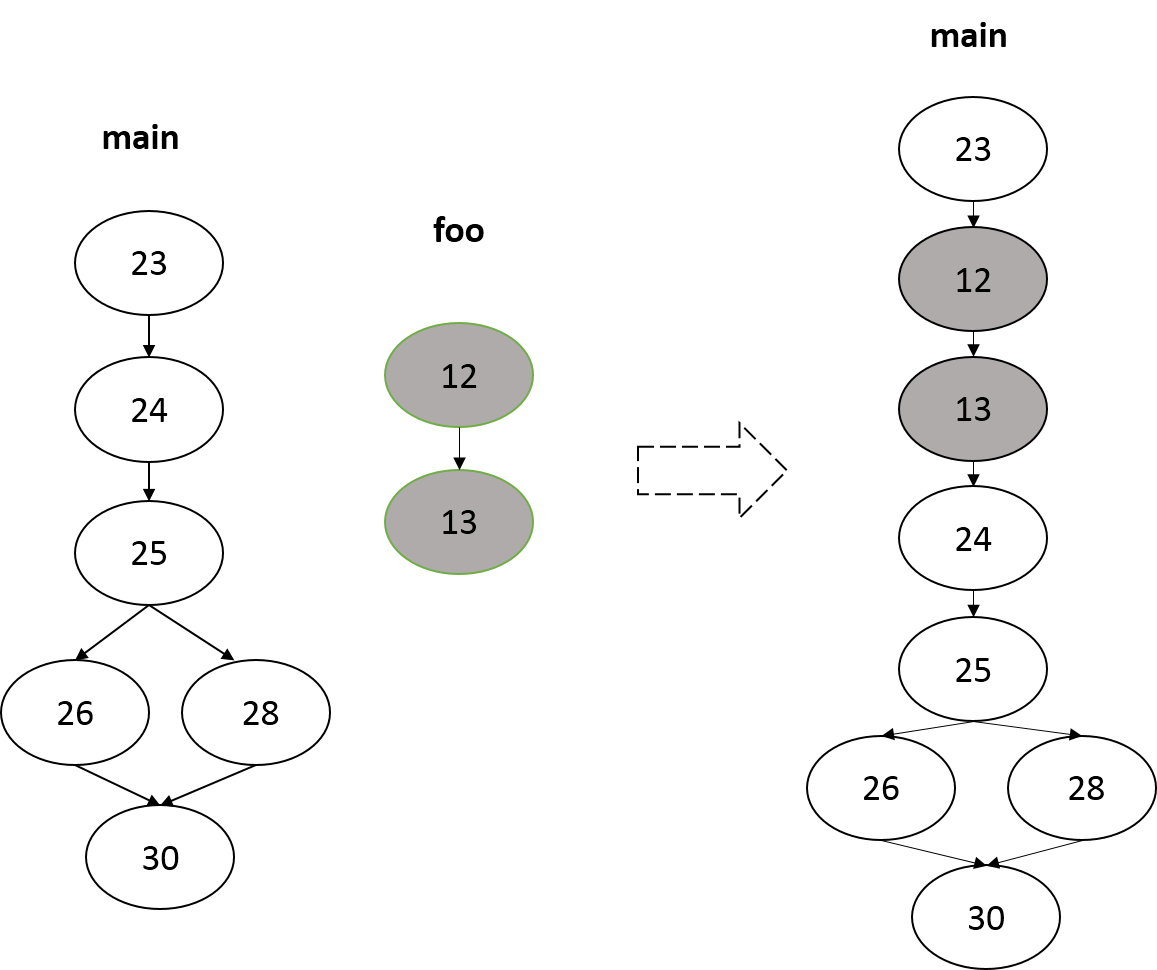
\includegraphics[width=0.70\textwidth]{figures/ICFG4-6}
	\caption{全局控制流图构建示例}\label{fig:figure4-6}
\end{figure}



\section{代码特征抽取}
分析域的全局控制流图可以表示空指针引用缺陷相关上下文代码的结构信息,但是代码不仅包含结构信息,还包含语义信息。本文构建的全局控制流图的结点为Jimple表示的Unit,它表示了一个抽象的语法层面的语句类型,以Unit为基本单位,本文选取了6个维度的信息进行编码作为该结点的特征附加在控制流图结构上,这些维度分别如下:

1.前驱结点数量

以上文构建的全局控制流图为基础,针对图中的每个结点获取其前驱结点的数量,作为该维度的特征值。

2.语句类型

Unit表示抽象的语句类型,实际上它包含了15种具体的Stmt语句类型,这些具体的语句类型和编码如表\ref{tab:table4-3}所示。

\begin{table}[hb]
	\centering
	\caption{Jimple中Stmt语句类型及特征编码} \label{tab:table4-3}
	\begin{tabular*}{0.9\textwidth}{@{\extracolsep{\fill}}ccc}
		\toprule[1pt]
		语句类别	&Stmt名称	&编码	 \\
		\midrule[1pt]
		\multirow{3}*{核心指令} &
		NopStmt	& 1	\\
		& IdentityStmt	& 2 \\
		& AssignStmt	&3 \\
		\specialrule{0em}{1pt}{1pt}
		\hline
		\specialrule{0em}{1pt}{1pt}
		
		\multirow{5}*{方法内控制流指令}	&
		IfStmt	& 4 \\
		& GotoStt	& 5 \\
		& BreakPointStmt	& 6 \\
		& TableSwitchStmt	& 7 \\
		& LookUpSwitchStmt	& 8 \\
		\specialrule{0em}{1pt}{1pt}
		\hline
		\specialrule{0em}{1pt}{1pt}
		\multirow{3}*{方法间控制流指令} &
		InvokeStmt	&9 \\
		& ReturnStmt	&10 \\
		& ReturnVoidStmt	&11 \\
		\specialrule{0em}{1pt}{1pt}
		\hline
		\specialrule{0em}{1pt}{1pt}
		\multirow{2}*{监视器指令} &
		EnterMonitorStmt	&12 \\
		& ExitMonitorStmt	&13 \\
		\specialrule{0em}{1pt}{1pt}
		\hline
		\specialrule{0em}{1pt}{1pt}
		\multirow{2}*{处理异常指令} &
		ThrowStmt	&14 \\
		& RetStmt	&15 \\
		\bottomrule[1pt]
	\end{tabular*}
\end{table}

3.调用语句类型

调用语句表明该程序涉及到了跨过程的分析,在Jimple包含的Stmt中,实现InvokeStmt接口的类有五种,它们表示五种调用方法的类型,它们的编码如表\ref{tab:table4-4}所示,如果该结点不包含方法调用语句,标记为0。

\begin{table}[hb]
	\centering
	\caption{Jimple中调用语句的类型及特征编码} \label{tab:table4-4}
	\begin{tabular*}{0.9\textwidth}{@{\extracolsep{\fill}}ccc}
		\toprule
		调用指令	&说明	&编码	 \\
		\midrule
		invokestatic & 调用静态方法	& 1	\\
		invokespecial & 调用私有方法、父类方法、构造方法	& 2 \\
		invokevirtual & 调用抽象方法	&3 \\
		invokeinterface	&调用接口方法 & 4 \\
		invokedynamic & 调用动态方法 	& 5 \\
		\bottomrule
	\end{tabular*}
\end{table}

4.使用的操作数数量

该维度特征表示了指令对操作数使用的密集程度,过多的操作数使用往往也代表着算术指令的密集使用。

5.空指针传递情况

如果当前节点涉及到了Null值的传递操作,可以说明下文中有更多可能会触发空指针引用异常。空指针的传递也有不同的方式需要编码,如表\ref{tab:table4-5}所示,如果没有发生空指针传递,编码为0。

\begin{table}[hb]
	\centering
	\caption{Jimple中空指针传递类型及特征编码} \label{tab:table4-5}
	\begin{tabular*}{0.9\textwidth}{@{\extracolsep{\fill}}ccc}
		\toprule
		空指针传递指令	&传递方式	&编码	 \\
		\midrule
		ReturnStmt & 方法返回值	& 1	\\
		InvokeStmt & 方法调用传参	& 2 \\
		definitionStmt & 直接赋值	&3 \\
		\bottomrule
	\end{tabular*}
\end{table}

6.空指针检查情况

空指针检查可以很好的避免下文中对空指针的引用,该语句通常会影响到工具检测结果的判定。如果该结点对Null值进行了检查,标记为1,否则为0;

通过六个维度的特征抽取,不仅可以体现全局控制流图的结构特征,而且可以体现图中每个结点即Jimple指令的语义特征。但是Java代码在转换为Jimple中间表示的过程中,为了使得到的语法单位都是标准的三地址表达式,将Java基本语句进行了大量的拆解重组,使得Jimple的基本语句的粒度比Java基本语句的粒度要小很多,这就使得生成的全局控制流图所能体现的特征更加不明显。为了让在模型训练的过程中更加容易的对代码分类,需要将生成的全局控制流图进一步压缩,使得图中每个结点接近基本块的维度。具体操作如算法\ref{alg:alg4-2}。

\begin{algorithm}%
	\LinesNumbered
	\KwIn{控制流图$G_c$}
	\KwOut{压缩后的控制流图$G_c'$}
	workList $\leftarrow \emptyset$  \\
	workList $\leftarrow \{G_c.RootNode\}$  \\
	\While{$worklist \neq \emptyset$}{
		node $\leftarrow$ workList.next \\
		remove node from workList \\
		node set visited \\
		\If{size of node.succList = 0}{
			node set visited \\
			continue \\
		}\ElseIf{size of node.succList = 1}{
			$tmpNode \leftarrow node$ \\
			\While{size of node.succList = 1}{
				$succNode \leftarrow node.succlist[0]$ \\
				\If{size of succNode.succList > 1 OR size of succNode.precList > 1}{
					break \\
				}
				mergeAttribute(tmpNode) \\
				$tmpNode \leftarrow succNode$ \\
				tmpNode set visited \\
			}
			$node.succList \leftarrow tmpNode.succList$ \\
			insert node into $G_c'$ \\
			\ForEach{succNode in node.succList}{
				\If{succNode is not visited}{
					insert succNode into workList \\
				}	
			}
		}\Else{
			\ForEach{succNode in node.succList}{
				\If{succNode is not visited}{
					insert succNode into workList \\
				}	
			}
		}
		insert node into $G_c'$ \\
	}
	\Return $G_c'$
	\caption{控制流图压缩算法}
	\label{alg:alg4-2}
\end{algorithm}

\begin{figure}
	\centering
	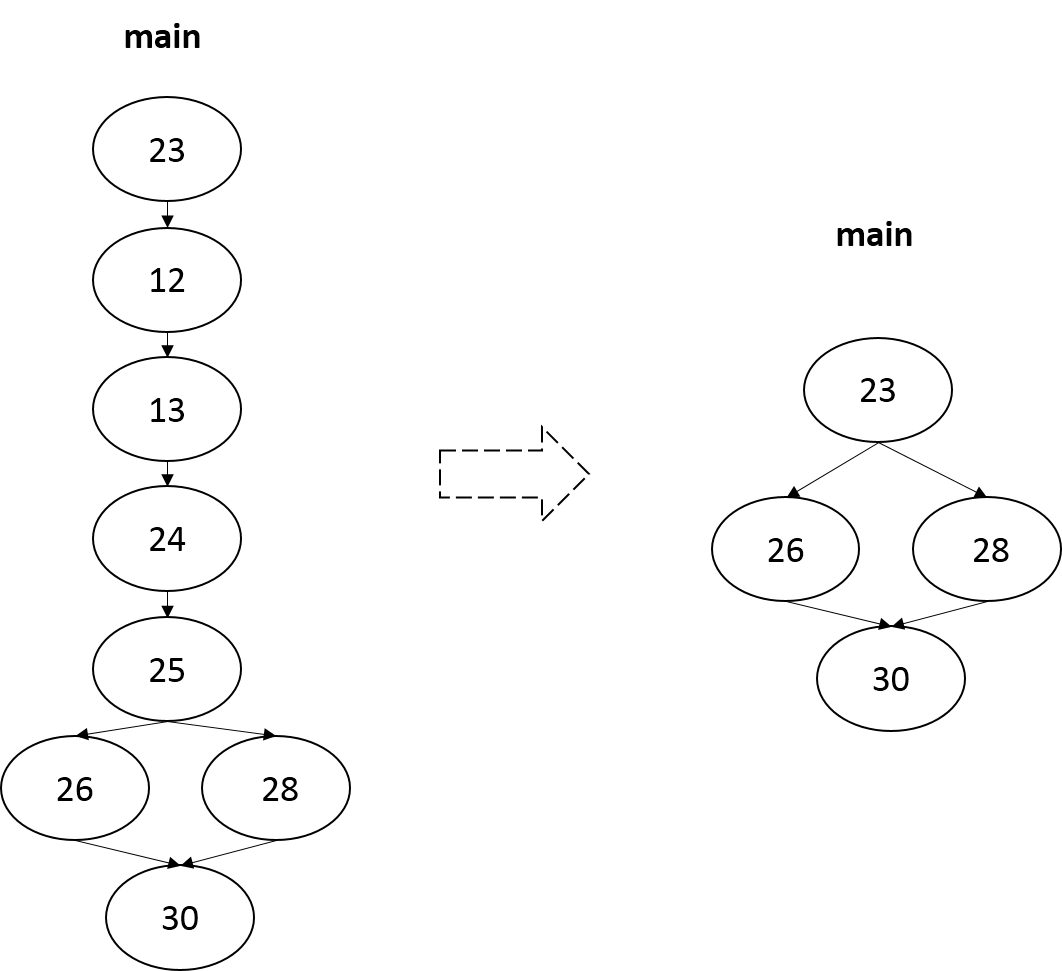
\includegraphics[width=0.70\textwidth]{figures/ICFG4-7}
	\caption{全局控制流图压缩示例}\label{fig:figure4-7}
\end{figure}


经过此算法处理,图\ref{fig:figure4-6}生成的全局控制流图将被进一步压缩,如图\ref{fig:figure4-7}所示。此算法将图中的串行结点,即前驱和后继结点数量均为1的结点合并为1个结点。同时,在算法的第16行进行了$mergeAttribute$的操作,这个操作可以将多个结点的特征属性转换到压缩后的一个结点上。具体转换方法如表\ref{tab:table4-6}所示,压缩后的图中结点的特征由压缩前多个结点的特征综合得到。

\begin{table}[hb]
	\centering
	\caption{控制流图压缩后的结点特征转换} \label{tab:table4-6}
	\begin{tabular*}{0.9\textwidth}{@{\extracolsep{\fill}}cc}
		\toprule
		压缩前特征值	&压缩后特征值	 \\
		\midrule
		前驱结点数量 & 压缩后结点的前驱结点数量	\\
		语句类型 & 被压缩结点中出现的语句类型的种类数量	 \\
		调用语句类型 & 被压缩结点中出现调用语句的数量 \\
		使用的操作数数量 & 被压缩结点中使用的操作数数量之和 \\
		调用语句类型 & 被压缩结点中调用语句的数量之和 \\
		调用语句类型 & 被压缩结点中调用语句的数量之和 \\
		\bottomrule
	\end{tabular*}
\end{table}

\section{数据标注}

\section{本章小结}